% ==========================================================================
%  Dipole geometry only  --  PHY 410/505, Assignment 2, P1
%  Compile:  pdflatex dipole-geometry.tex   (standalone -> cropped PDF)
% ==========================================================================
\documentclass[border=8pt]{standalone}
\usepackage{amsmath}
\usepackage{tikz}
\usetikzlibrary{arrows.meta}

\def\ax{x}                                  % <-- axis / distance symbol

\definecolor{poscol}{RGB}{178, 34, 34}
\definecolor{negcol}{RGB}{28, 68, 158}

\begin{document}
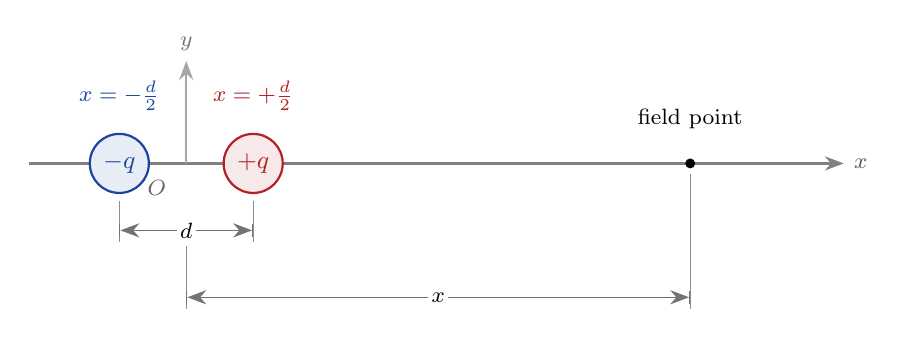
\begin{tikzpicture}[
  >={Stealth[length=2.4mm]},
  chgp/.style={circle,thick,draw=poscol,text=poscol,fill=poscol!10,
               minimum size=7.5mm,inner sep=0pt,font=\small},
  chgm/.style={circle,thick,draw=negcol,text=negcol,fill=negcol!10,
               minimum size=7.5mm,inner sep=0pt,font=\small},
  dimline/.style={|<->|,thin,black!55},
  lbl/.style={font=\footnotesize},
]

  % --- axes ---
  \draw[->,thick,black!50] (-2.0,0) -- (8.35,0) node[right,lbl,black!65] {$\ax$};
  \draw[->,thick,black!35] (0,0) -- (0,1.30) node[above,lbl,black!55] {$y$};
  \node[lbl,black!60,anchor=north east] at (-0.13,-0.09) {$O$};

  % --- charges ---
  \node[chgm] (qm) at (-0.85,0) {$-q$};
  \node[chgp] (qp) at ( 0.85,0) {$+q$};
  \node[lbl,negcol,anchor=south] at (-0.85,0.55) {$\ax=-\tfrac{d}{2}$};
  \node[lbl,poscol,anchor=south] at ( 0.85,0.55) {$\ax=+\tfrac{d}{2}$};

  % --- field point ---
  \fill[black] (6.40,0) circle (1.8pt);
  \node[lbl,anchor=south] at (6.40,0.32) {field point};

  % --- separation d ---
  \draw[black!45,thin] (-0.85,-0.48) -- (-0.85,-1.00);
  \draw[black!45,thin] ( 0.85,-0.48) -- ( 0.85,-1.00);
  \draw[dimline] (-0.85,-0.85) -- (0.85,-0.85);
  \node[lbl,fill=white,inner sep=1.2pt] at (0,-0.85) {$d$};

  % --- distance to the field point ---
  \draw[black!45,thin] (0,-1.05) -- (0,-1.85);
  \draw[black!45,thin] (6.40,-0.14) -- (6.40,-1.85);
  \draw[dimline] (0,-1.70) -- (6.40,-1.70);
  \node[lbl,fill=white,inner sep=1.2pt] at (3.20,-1.70) {$\ax$};

\end{tikzpicture}
\end{document}
